\setcounter{rownumber}{0}
\chapter{Laser Cooling of Traveling-Wave Phonons in an Optical Fiber}
\label{ch:Cooling}
\acresetall

Joel N. Johnson\footnote{\label{Cooling-NAU}
Department of Applied Physics and Materials Science, Northern Arizona University, Flagstaff, AZ 86011, USA}%
\textsuperscript{,}\footnote{\label{Cooling-MIRA}
Center for Materials Interfaces in Research and Applications, Flagstaff, AZ 86011, USA},
Danielle R. Haverkamp\textsuperscript{\ref{Cooling-NAU},\ref{Cooling-MIRA}},
Yi-Hsin Ou\footnote{\label{Cooling-UofA}
College of Optical Sciences, University of Arizona, Tucson, AZ, USA},
Khanh Kieu\textsuperscript{\ref{Cooling-UofA}},
Nils T. Otterstrom\footnote{\label{Cooling-Sandia}
Photonic and Phononic Microsystems, Sandia National Laboratories, Albuquerque, New Mexico, USA},
Peter T. Rakich\footnote{\label{Cooling-Yale}
Department of Applied Physics, Yale University, New Haven, CT, USA},
Ryan O. Behunin\textsuperscript{\ref{Cooling-NAU},\ref{Cooling-MIRA}}

\hfill

\textit{This chapter elaborates on experiments and results related to the demonstration of optomechanical cooling of traveling wave phonons in optical fiber which have been published as an article by the same name in Physical Review Applied by Johnson et al. (2023) \cite{johnson2023laser}. Any discrepancies, omissions, or errors that may exist between the published paper and this dissertation chapter are the sole responsibility of the author, as the text, analyses, and interpretations herein represent an independent and original presentation of the work.}

%--------------------------------------------------------------------%

\section{Introduction}
\label{Cooling:sec:Introduction}

Materials above the ground state experience therodynamic variations such as temperature and density. These thermal fluctuations alter the optical properties of a given material, allowing a scattering process to occur (see Section \ref{Introduction:sec:LightScattering}). Spontaneous Brillouin scattering is the inelastic scattering of light with these thermal fluctuations within a material, facilitating an energy exchange between the optical and acoustic domains. While a given medium typically supports a multitude of thermally excited acoustic modes (including both transverse and longitudinal modes) we focus here specifically on longitudinally travelling acoustic waves to demonstrate cooling in a continuous (non-resonant) system.

[lit review, state of the art]

%--------------------------------------------------------------------%

\section{Optomechanical Cooling and Heating}
\label{Cooling:sec:CoolingandHeating}

\subsection{Physical Mechanism}
\label{Cooling:subsec:PhysicalMechanism}

Backward Brillouin scattering targets longitudinally traveling acoustic waves (or phonons) through two complementary processes---Stokes and anti-Stokes, illustrated in Figures \ref{fig:Cooling:StokesHeating} and \ref{fig:Cooling:anti-StokesCooling}, respectively. In the Stokes process, an incident photon of frequency \(\omega\) scatters with a \textit{retreating} phonon of frequency \(\Omega\) annihilating the \textit{photon} and creating both an additional phonon of frequency \(\Omega\) and a backscattered photon at the difference energy (\(\omega_{\mathrm{Stokes}} = \omega - \Omega\)). In this way, both energy and momentum are conserved. This can be visualized by an analogy, in which the incident light experiences a doppler \textit{down}-shift in frequeny as though the photon were reflected from a retreating mirror. Since this processes results in an increase in the phonon population within the respective longitudinal mode of the material, this process is referred to as optomechanical heating. The energy lost by the light is gained by the material in the form of mechanical vibrations.

\begin{figure}[t]
    \centering
    \begin{subfigure}[b]{0.49\textwidth}
        \centering
        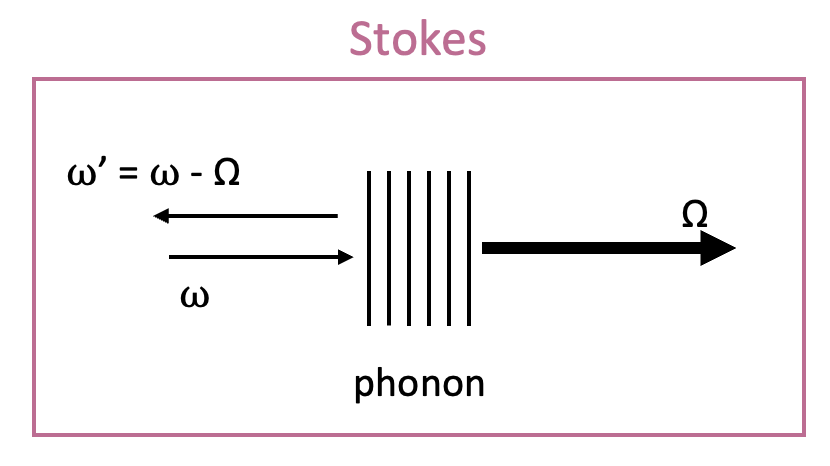
\includegraphics[width=\textwidth]{figs/3-Cooling/StokesHeatingProcess.png}
        \caption{}
        \label{fig:Cooling:StokesHeating}
    \end{subfigure}
    \hfill
    \begin{subfigure}[b]{0.49\textwidth}
        \centering
        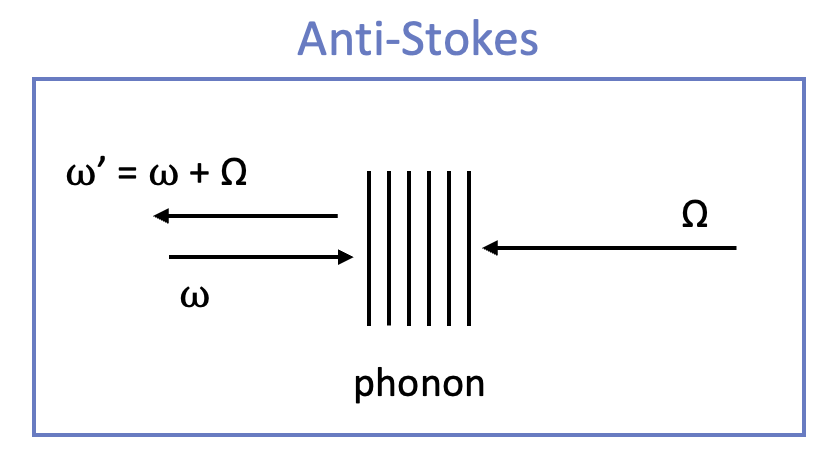
\includegraphics[width=\textwidth]{figs/3-Cooling/anti-StokesCoolingProcess.png}
        \caption{}
        \label{fig:Cooling:anti-StokesCooling}
    \end{subfigure}
    \caption{Illustration of optomechanical heating and cooling processes. Figure \ref{fig:Cooling:StokesHeating} shows an incident photon of frequency \(\omega\) scattering with a retreating phonon of frequency \(\Omega\), resulting in the annihilation of the incident photon and the creation of both an additional retreating phonon of frequency \(\Omega\) and a backwards propagating photon of reduced frequency and thereby energy (\(\omega_{\mathrm{Stokes}} = \omega - \Omega\)). Figure \ref{fig:Cooling:anti-StokesCooling} shows the inverse process, whereby an incident photon, \(\omega\), scatters with an approaching phonon, \(\Omega\), annihilating the incident photon and the phonon to produce a backwards propagating photon of increased frequency and thereby energy (\(\omega_{\mathrm{anti-Stokes}} = \omega + \Omega\)).}
    \label{fig:Cooling:StokesProcesses}
\end{figure}

The anti-Stokes process is the inverse process, whereby an \textit{approaching} phonon of frequency \(\Omega\) scatters with an incident photon of frequency \(\omega\), annihilating the \textit{phonon} and creating a backscattered photon at the addition energy (\(\omega_{\mathrm{anti-Stokes}} = \omega + \Omega\)). Both energy and momentum are again conserved, however in the anti-Stokes process, the incident light experiences a doppler \textit{up}-shift in frequency as if, to continue the analogy, the photon were reflected from an approaching mirror.

\subsection{Spectral Signatures of Cooling and Heating}
\label{Cooling:subsec:SpectralSignaturesofCoolingandHeating}

Spectral amplitude provides a measure of the power of the backscattered light, increasing with both pump power \(P_{\mathrm{P}}\) as well as temperature \(T\) of the phonon mode (see Equation~\ref{eq:sponBSscatteredPower} in Appendix~\ref{appendix:comparison}). As a result, both Stokes and anti-Stokes spectral amplitudes increase with increasing pump power, but at inequal rates respective of pump power. With increasing pump power, the anti-Stokes scattering process serves to cool the anti-Stokes phonon mode, partially discounting the scattered power of the anti-Stokes light collected by the detector. The simultaneous Stokes process experiences an inverse effect, whereby increasing pump power serves to heat the Stokes phonon mode, contributing to an increase in scattered power of Stokes light collected by the detector. The overall effect of these processes is a sublinear growth in amplitude of the anti-Stokes spectrum and superlinear growth of the Stokes spectrum.

\section{Methods}
\label{Cooling:sec:Methods}

While spontaneous Brillouin scattering processes naturally alter phonon populations (and thus mode temperatures), practical demonstration and detection of these effects pose significant challenges. Foremost among these is the requirement to remain in the spontaneous regime: we wish to probe the natural thermal phonons in a medium, so we cannot rely on artificially driving the mechanical modes to enhance scattered power (see Appendix~\ref{appendix:comparison}, and specifically Figure~\ref{fig:SponBSvsStimBSvsCoBS}, for a comparison of scattered power produced by different Brillouin techniques). Although stimulated Brillouin scattering (SBS) is often employed to boost signal levels, it actively drives phonon populations via injected optical fields, and thus no longer measures the intrinsic thermal phonons. In practical terms, SBS occurs when the overall process gain factor \(G = G_{\mathrm{B}}P_{\mathrm{P}}L\) (where \(G_{\mathrm{B}}\) is the effective Brillouin gain, \(P_{\mathrm{P}}\) the pump power, and \(L\) the effective length) far exceeds unity (\(G \gg 1\)).

To demonstrate optomechanical cooling (i.e., an anti-Stokes process that lowers phonon energy), one must detect scattered light from a mode whose phonon population has been reduced. This is intrinsically difficult because a decreased phonon population means fewer scattering events, and hence diminished backscattered light. Consequently, an ideal testbed should provide sufficiently high single-pass gain (overall gain factor near unity) to enable clear detection, yet remain below the threshold that would drive the process into the stimulated regime. Achieving this balance ensures that measurements reflect genuine spontaneous cooling of a thermally populated phonon mode, rather than an artifact of optically driven phonons.

In addition to the requirement that the overall process gain be near but below unity, temporal constraints impose further critical conditions. Specifically, the rate at which phonons are removed from the system must exceed the rate at which they are replenished by the thermal bath to ensure net cooling of the anti-Stokes mode. This condition demands that backscattered photons leave the system rapidly, carrying away the extracted mechanical energy. A mean-field analysis (see Appendix~A of Johnson et al. (2023) \cite{johnson2023laser}) shows that the relevant depletion rate is \(4v_{\mathrm{g}}/L\), where \(v_{\mathrm{g}}\) is the group velocity of the anti-Stokes light and \(L\) is the system length. This must exceed the mechanical dissipation rate \(\Gamma_{\mathrm{0}}\), which represents the natural return of the phonon mode to thermal equilibrium. Hence, a suitable platform for demonstrating optomechanical cooling of traveling-wave phonons must fulfill the fast escape condition \(4v_{\mathrm{g}}/L > \Gamma_{\mathrm{0}}\). Meeting this requirement on system length, however, directly conflicts with the desire for a sufficiently high overall gain factor, illustrating the delicate balance needed for effective cooling.

%--------------------------------------------------------------------%

\subsection{\texorpdfstring{$CS_{2}$}{CS2}-Filled Liquid-Core Optical Fiber}
\label{Cooling:subsec:CS2FilledLCOF}

\begin{figure}[t]
  \centering
  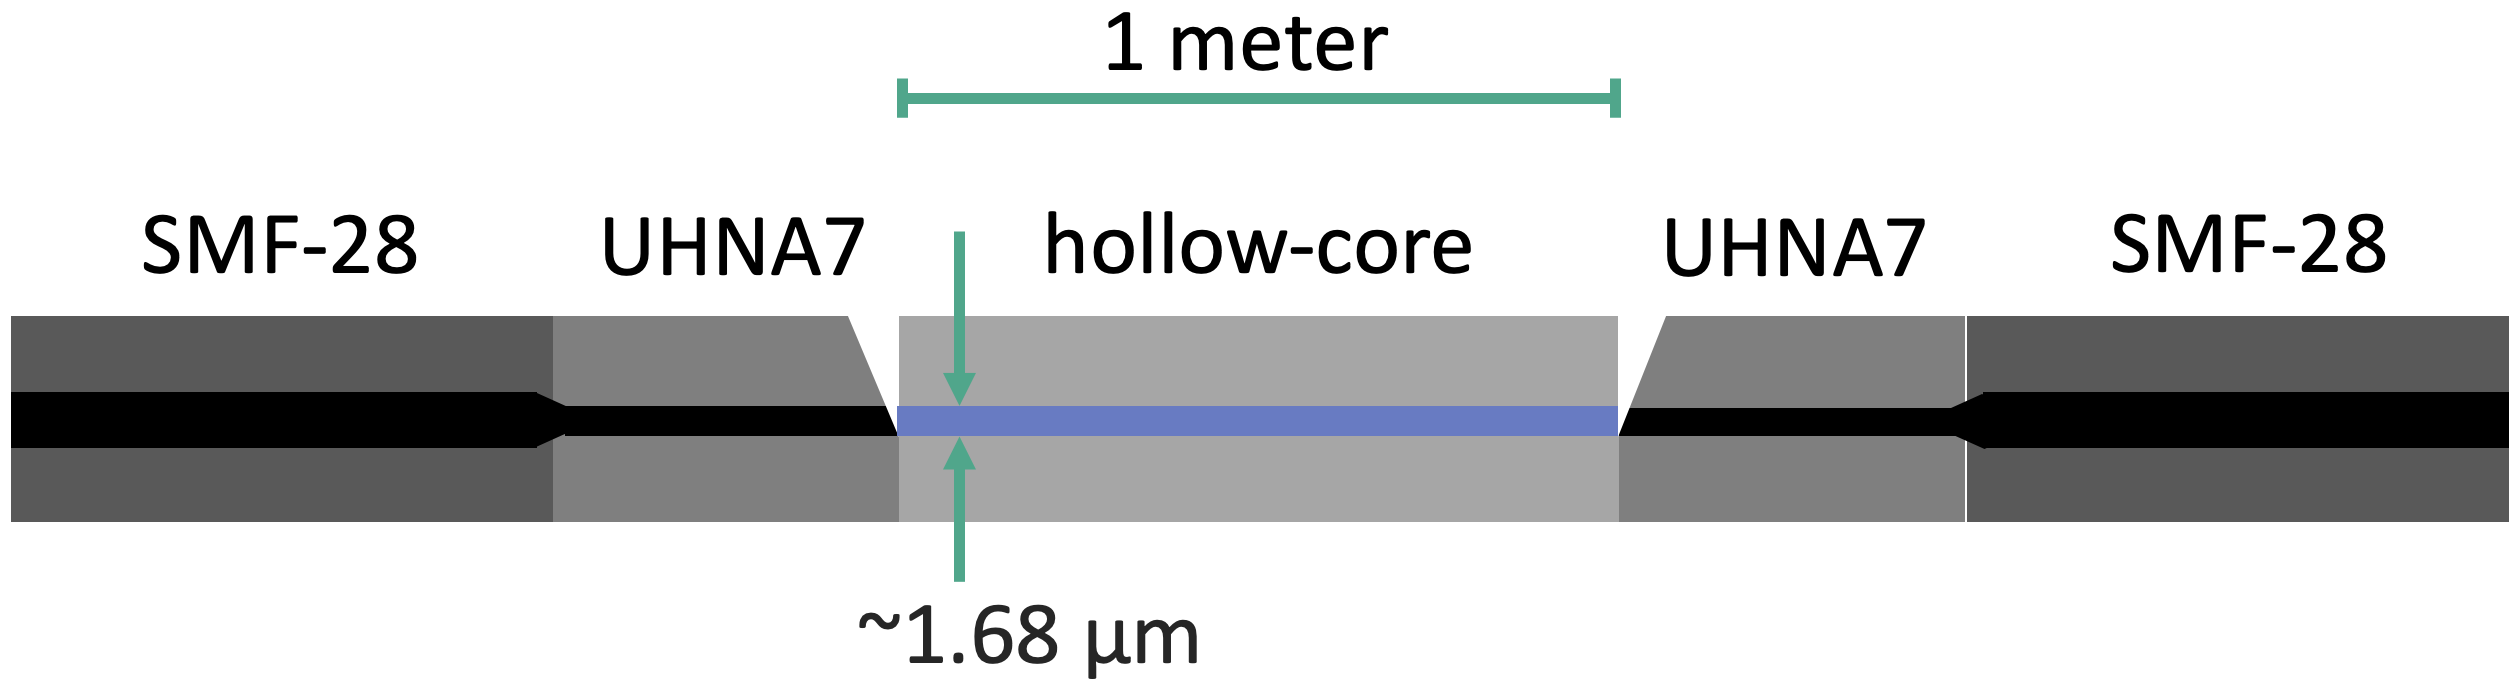
\includegraphics[width=\textwidth]{figs/3-Cooling/LCOFdiagram.png}
  \caption{Schematic of \ac{LCOF} design. A length of \ac{SMF-28} is arc-spliced to 5-\SI{10}{\centi\meter} of \ac{UHNA7} fiber, with a post-arc process applied to taper the larger \ac{SMF-28} core down to the smaller \ac{UHNA7} core for better mode matching and coupling efficiency. The \ac{UHNA7} fiber is angle-cleaved and fusion-spliced to a flat-cleaved hollow-core fiber via a heated filament in a Vytran fusion splicer system. The angle cleave results in a splice that only partially fuses the two fibers, leaving a pathway for liquid to enter the hollow core fiber via capillary action once submerged. A mirrored splice configuration on the other end of the length of hollow-core fiber allows air to escape as the fiber fills, and a reverse taper again provides improved mode matching for the light to recouple into \ac{SMF-28}.}
  \label{fig:LCOF diagram}
\end{figure}

To demonstrate optomechanical cooling of traveling wave phonons, we utilize \SI{1}{\meter} of \acl{LCOF} filled with carbon disulfide, first developed by Kieu et al. (2012). \cite{kieu2012integrated} This platform features large optomechanical coupling due to the high electrostritive response of \ce{CS2} \cite{boyd2020nonlinear} and the small effective area defining acousto-optic mode overlap offered by the small \SI{0.9}{\micro\meter} core radius of the capillary fiber. These characteristics of the \ac{LCOF} system combine to produce an effective Brillouin gain coefficient \(G_{\mathrm{B}} \sim\)\SI{2.3}{\per\watt\per\meter}, enabling sufficient scattering within the relatively short length required to satisfy the fast-escape condition \(4v_{\mathrm{g}}/L > \Gamma_{\mathrm{0}}\) (\(4v_{\mathrm{g}}/L \approx\) \SI{0.82}{\giga\hertz} and \(\Gamma_{\mathrm{0}} \approx\) \SI{0.61}{\giga\hertz}). \cite{johnson2023laser} Additionally, this \ce{CS2}-filled \ac{LCOF} system provides excellent acoustic and optical guidance due to the large electromagnetic and acoustic impedance differential between the \ce{CS2} core and surrounding silica. \cite{behunin2019spontaneous}

Figure~\ref{fig:LCOF diagram} shows a schematic of the \ac{LCOF} design. Coupling into and out of the \ac{LCOF} is facilitated by a short length of tapered \ac{UHNA7} for better mode matching between the \SI{4.8}{\micro\meter} core radius \ac{SMF-28} and the \SI{0.84}{\micro\meter} core radius of the capillary fiber. An angled cleave of the \ac{UHNA7} fiber allows for a small wedge gap to remain after fusion splicing to the capillary fiber. This gap allows liquid \ce{CS2} to enter and fill the hollow core of the capillary fiber via capillary action. Appendix~\ref{Cooling:Appendix:sec:FabricationofCS2FilledLCOF} describes the fabrication and filling processes of the \ac{LCOF} and details key insights which contributed to significant reductions in failure rate as well as time and material cost of sample preparation.

%--------------------------------------------------------------------%

\subsection{Experiment A: Spontaneous Brillouin Cooling}
\label{Cooling:subsec:ExperimentASpontaneousBrillouinCooling}

We conducted two independent experiments to demonstrate and verify laser cooling of traveling wave phonons in our \ce{CS2}-\ac{LCOF} platform. The first experiment employed a pump laser to inject \SI{1.55}{\micro\meter} light into the \ac{LCOF} and the frequency-shifted backscattered Stokes and anti-Stokes light was filtered and collected by a detector. In this experiment, evidence of cooling is given by symmetry breaking of the amplitudes and widths of the Stokes and anti-Stokes spectra as pump power increases.

Figure~\ref{fig:Cooling:ExperimentADesign} shows a schematic diagram of the experimental setup for Experiment~A. A \ac{CW} pump laser emitting at \SI{1.55}{\micro\meter} (\(\omega_{P}\)) is amplified by an \ac{EDFA} and its power is controlled by a \ac{VOA}. This light is subsequently routed via a circulator to the \ce{CS2}-\ac{LCOF}, where some of the light backscatters within the length of the \ac{LCOF}. Backscattered light is frequency-shifted, up for anti-Stokes (\(\omega_{\mathrm{aS}} = \omega_{\mathrm{P}} + \Omega_{\mathrm{B}}\)) and down for Stokes
(\(\omega_{\mathrm{S}} = \omega_{\mathrm{P}} - \Omega_{\mathrm{B}}\)),
by a frequency band centered around the Brillouin frequency of the \ac{LCOF} (\(\Omega_{\mathrm{B,\,LCOF}} \approx\) \SI{2.25}{\giga\hertz}). Backscattered light is routed by circulators to a \SI{5}{\giga\hertz} \ac{BPF} to allow selection of either the Stokes or anti-Stokes light while also reducing unwanted frequency noise. The filtered signal is then incident on a photodiode detector sensitive to \si{\giga\hertz} frequencies. A \ac{LO} is synthesized from the pump laser, polarization controlled, amplified, and combined with the signal pre-detector for heterodyne detection. Output from the detector is amplified with a \ac{RF} amplifier and sent to a \ac{RFSA} for data collection.

To conduct the experiment, pump power was varied from \SI{10}{\milli\watt} to \SI{290}{\milli\watt} in increments of \SI{10}{\milli\watt}, as measured pre-injection into the \ac{LCOF}, and respective Stokes and anti-Stokes spectra for each pump power were collected sequentially by tuning the placement of the \ac{BPF}. Optical transmission through the entire \ac{LCOF} sample which was used for the published data was measured to be 17\%, giving \(100\sqrt{0.17} \approx 41\%\) transmission through just the first splice assuming equal transmission through both \ac{LCOF} splices. This provides a scaling factor for obtaining intrafiber powers from injected pump power (\(P_{\mathrm{intrafiber}} = \sqrt{0.17}P_{\mathrm{P}}\)) which was used for data processing and analysis.

\begin{figure}[t]
  \centering
  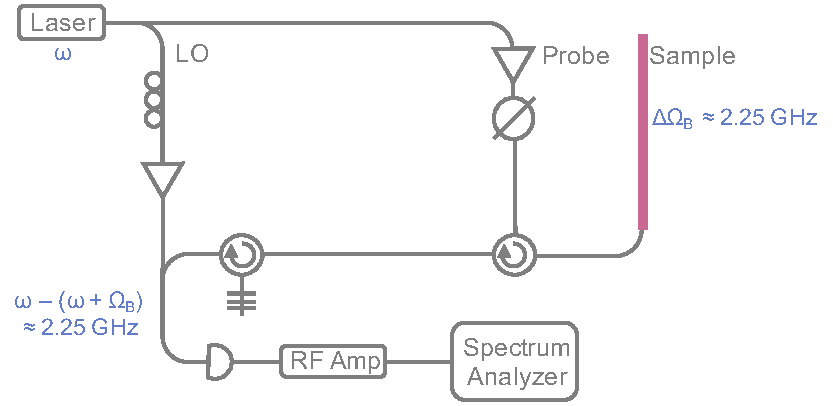
\includegraphics[width=\textwidth]{figs/3-Cooling/pumpOnlyDesign.pdf}
  \caption{Schematic of experimental setup for Experiment~A. In this experiment, a \ac{CW} pump laser emitting at \SI{1.55}{\micro\meter} is amplified, passed through a circulator, and injected into the \ce{CS2}-\ac{LCOF}. Backscattered light is routed to a \ac{BPF} for selection of Stokes or anti-Stokes frequencies and sent to a detector. A \ac{LO} is synthesized from the pump laser for heterodyne detection, whereby a \acl{PC} is used to align the polarization of the \ac{LO} to that of the backscattered signal. The signal passes through a \acl{RF} amplifier before being sent to a \ac{RFSA} for collection. Pump power is controlled by a \ac{VOA} just after the \ac{EDFA}.}
  \label{fig:Cooling:ExperimentADesign}
\end{figure}

\subsection{Experiment B: Pump-Probe Verification}
\label{Cooling:subsec:ExperimentBPump-ProbeVerification}

\begin{figure}[t]
  \centering
  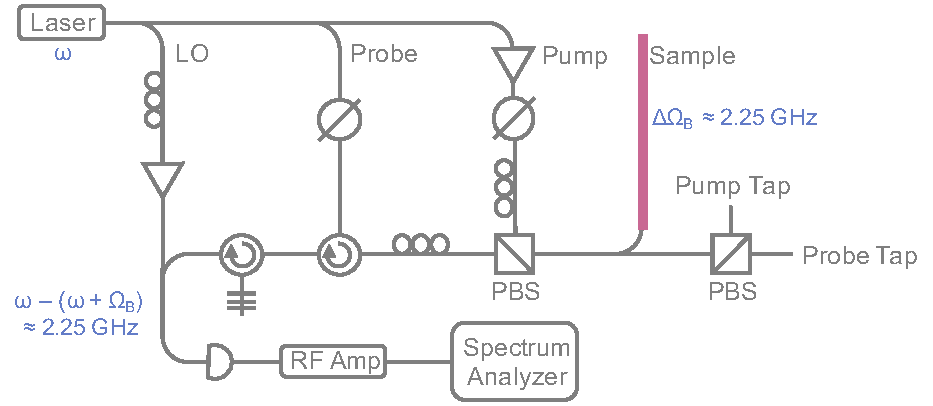
\includegraphics[width=\textwidth]{figs/3-Cooling/pumpProbeDesign.pdf}
  \caption{Schematic of experimental setup for Experiment~B.}
  \label{fig:Cooling:ExperimentBDesign}
\end{figure}

A second experiment was conducted to provide direct evidence of cooling via a pump-probe technique whereby a separate probe laser is held at constant power while a pump laser is varied to affect cooling in the \ac{LCOF}. In this pump-probe experiment, backscattered light from the probe laser provides direct evidence of cooling through spectral changes in amplitude and width as pump power increases.

%--------------------------------------------------------------------%

\section{Results}
\label{Cooling:sec:Results}


\subsection{Experiment A Results}
\label{Cooling:subsec:ExperimentAResults}



% need for normalized cooling metric - per pump power, and such that one cannot start a system in a heated state to achieve a greater stated cooling ability. Or maybe room temperature is identical across systems? check. if not, normalize.

\subsection{Experiment B Results}
\label{Cooling:subsec:ExperimentBResults}

%--------------------------------------------------------------------%

\section{Discussion}
\label{Cooling:sec:Discussion}

\subsection{Pathways to Net Cooling}
\label{Cooling:subsec:PathwaystoNetCooling}

Ideas to achieve net cooling, one might design a system where:

1) single pass gain bias
     swing energy transfer bias to favor anti-Stokes over Stokes (mode-dependent gain)
     the Stokes process were not permitted (ryan's only idea), or just significantly restricted - what is that bias threshold requirement?
     currently, we are net *heating* the system because it is easier to heat from equilibrium than cool (right? explore this. it's also hard to make it hotter beyond a certain point.)
     implementation ideas:
       multi-pump scheme to destructively interfere with Stokes and/or constructively interfere with anti-Stokes
       doping or specialized waveguide gratings that pick out the Stokes band for out-of-plane scattering

2) time bias
     create an energy transfer *rate* bias between Stokes and anti-Stokes
     can be accomplished with either the brillouin energy transfer rate or the repopulation rate

       brillouin process rate:
         4vg/L, have either group velocity or length be different for Stokes vs anti-Stokes (smaller vg or larger L for Stokes than anti-Stokes)
         make anti-Stokes fast light and/or Stokes slow light
         vg inversely proportional to pump power, so it's a balance
           increasing pump power = slower escape time (4vgL), and also larger dissipation (Gamma+)

       repopulation rate:
         thermally insulate the anti-Stokes mode from the thermal bath that would repopulate it
         or at least insulate it some amount more than Stokes (what is that threshold? even if it's only net cooled for picoseconds, what is that minimum crossover point insulation bias point)
         essentially locks in the cooled mode while letting the heated mode spill out
         implementation idea:
           design a fiber/waveguide with acoustic directional bias, such that phonons travelling one direction dissipate quicker because of the geometry/acoustic properties of the fiber. (triangles? acting as tapered acoustic dissipators, pointing in one direction?)

3) starting temperature
     Could you acieve net cooling in a cheap and dirty sense by starting the system in a very heated state, thus invoking a natural dissipation rate bias?! - yes!
     Things do naturally run hot, perhaps no extra fancy engineering is needed for some practical systems? (data processing, reduce thermal noise from above ambient heat)
     not traditional definition of optical refrigeration below ambient/thermal bath, but still *useful*
     is this already done? lit search

Think about a practical device or system for each of these cases (think waveguide playground!)

\subsection{Applications to Ground State Cooling}
\label{Cooling:subsec:ApplicationstoGroundStateCooling}


\subsection{Standardized Cooling Metric}
\label{Cooling:subsec:StandardizedCoolingMetric}


\subsection{Alternative Platforms}
\label{Cooling:subsec:AlternativePlatforms}

Tapered chalcogenide Photonic Crystal Fiber: Max Plank Results
